\documentclass[10pt]{article}

% Manage page layout
\usepackage[margin=2.5cm, includefoot, footskip=30pt]{geometry}
\pagestyle{plain}
\setlength{\parindent}{0em}
\setlength{\parskip}{1em}
\renewcommand{\baselinestretch}{1}

\usepackage{blkarray}
\usepackage{multirow}
\usepackage{amsmath}
\usepackage{amsfonts}
\usepackage{enumerate}
\usepackage{tikz}
\usetikzlibrary{calc}
% Node styles
\tikzset{
    % Two node styles for game trees: solid and hollow
    solid node/.style={circle,draw,inner sep=1.5,fill=black}, hollow node/.style={circle,draw,inner sep=1.5}
    }

\title{\textbf{Week 8.} Static games with incomplete information}
\date{}

\begin{document}
\maketitle


\subsection*{Bonus 1: Volunteer's dilemma with correlated costs}

Consider the volunteer's dilemma with payoffs

\begin{equation*}
    \begin{blockarray}{ccc}
        & C & D \\
        \begin{block}{c(cc)}
            C & (1 - c_1, 1 - c_2) & (1 - c_1, 1) \\
            D & (1, 1 - c_2) & (0, 0) \\
        \end{block}
    \end{blockarray}
\end{equation*}

Suppose \(c_1\) is randomly drawn from \([0, 2]\) uniformly. For \(c_2\) assume
that it is (anti-) correlated, such that \(c_1 + c_2 = 2\) is always satisfied
(whenever player 1 has a comparably high cost they know player 2 has a
comparable low cost). \textbf{Show that the following strategies are Bayesian Nash
equilibrium.}

\begin{equation*}
    S^{(1)}(c_1) = 
    \begin{cases}
        C,& \text{if } c_1 \leq 1\\
        D,              & \text{if } c_1 > 1
    \end{cases} \qquad
    S^{(2)}(c_2) = 
    \begin{cases}
        C,& \text{if } c_2 < 1\\
        D,              & \text{if } c_2 \geq 1
    \end{cases}
\end{equation*}

\underline{\textbf{Bonus question:}} Are there any other Bayesian Nash equilibria?


[Hint: To show that (\(S^{(1)}\), \(S^{(2)}\)) is a Bayesian Nash equilibrium,
consider player 1. Show that for $c_1 < 1$ and for $c_1 > 1$ the player
has no reason to deviate from \(S^{(1)}\). Do the same for player 2.]

\subsection*{Bonus 2: Second-price sealed bid auction}

An items is sold to the higher bid among \(n\) players. The players' values for
the item, \(\mathbf{v}^{(i)}\), are uniformly and independently drawn from \([0, 1]\).
The players' strategy is to choose a bid, depending on how much the item would be
worth to them, \(s^{(i)}: \mathbf{v}^{(i)} \rightarrow b^{(i)}\).

The player with the highest bid wins the auction. However, they only have to
pay the second-highest bid.

\begin{equation*}
\text{Payoff: }    \pi^{(i)} (b^{(i)}, b^{(-i)}) = 
    \begin{cases}
        \mathbf{v}^{(i)} - \max\limits_j(b^{(j)}), & \text{if } b^{(i)} > b^{(j)} \ \forall \ j \neq i \\
        (\mathbf{v}^{(i)} - \max\limits_{j \neq i}(b^{(j)})) / K, & \text{if } b^{(i)} = \max\limits_{j \neq i} (b^{(j)}) \ \& \ K \text{number of highest biddings}\\
        0,              & \text{otherwise}.
    \end{cases}
\end{equation*}

\textbf{Show that the strategy \(b^{(i)} = v^{(i)}\) weakly dominates any other
strategy.}

[Hint: Consider 3 cases. The first case is that \(\textbf{v}^{(i)} > \max\limits_j (b^{(j)})\).
Show that bidding \(b^{(i)} \neq \textbf{v}^{(i)}\) never yields a higher payoff than bidding
\(b^{(i)} = \textbf{v}^{(i)}\), but sometimes the payoff is worse. Similar for the cases
\(\textbf{v}^{(i)} = \max\limits_j (b^{(j)})\) and \(\textbf{v}^{(i)} < \max\limits_j (b^{(j)})\).]


\subsection*{Exercise 1: Revenue equivalence theorem}

Consider an auction between two players with valuations for an item again uniformly
drawn from \([0, 1]\). We already know the equilibria of the


\begin{itemize}
    \item first-price sealed bid auction: \(b ^ {(i)} =  \frac{1}{2} \textbf{v}^{(i)}\) (Example 4.5), and the
    \item second-price sealed bid auction: \(b ^ {(i)} =  \textbf{v}^{(i)}\) (Exercise 2).
\end{itemize}

\textbf{Show that the expected revenue for the seller (the price the winning bidding
has to pay) is the same for both auctions.}

[Hint: Suppose the player with the highest valuation assigns a value
\(\textbf{v}\) to the item. Show that the expected revenue of the seller is
\(\frac{\textbf{v}}{2}\), in both cases.]


\subsection*{Exercise 2: Pooling equilibrium of the IMPRS game}

Revisit the IMPRS game from Example 4.8. 

\begin{figure*}[!htbp]
    \begin{center}
    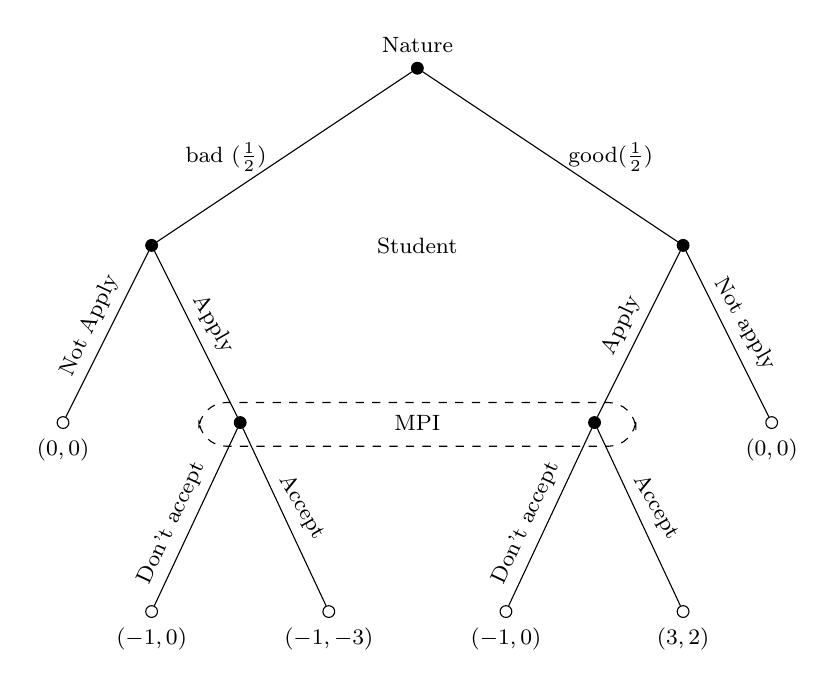
\begin{tikzpicture}[scale=1.5,font=\footnotesize] % Specify spacing for each level of the tree
        \tikzstyle{level 1}=[level distance=15mm,sibling distance=45mm] \tikzstyle{level 2}=[level distance=15mm,sibling distance=15mm]
        \tikzstyle{level 3}=[level distance=16mm]
        % The Tree
        \node(0)[solid node,label=above:{Nature}]{}
        child{node(1)[solid node]{}
        child{node[hollow node,label=below:{$(0, 0)$}]{} edge from parent node[above, rotate=65]{Not Apply}} 
        child{node[solid node]{} child{node(3)[hollow node, label=below:{$(-1, 0)$}]{} edge from parent node[above, rotate=65, xshift=-0.2cm]{Don't accept}} 
        child{node[hollow node, label=below:{$(-1, -3)$}]{} edge from parent node[above, rotate=-60]{Accept}} 
        edge from parent node[above, rotate=-60]{Apply}} 
        edge from parent node[left,xshift=-3]{bad $(\frac{1}{2})$}
            }
        child{node(2)[solid node]{}
        child{node[solid node]{}  child{node(4)[hollow node, label=below:{$(-1, 0)$}]{} edge from parent node[above, rotate=65, xshift=-0.2cm]{Don't accept}} 
        child{node[hollow node, label=below:{$(3, 2)$}]{} edge from parent node[above, rotate=-60]{Accept}} 
        edge from parent node[above, rotate=65]{Apply}} 
        child{node[hollow node,label=below:{$(0, 0)$}]{} edge
        from parent node[above, rotate=-60]{Not apply}} edge from parent node[right,xshift=3]{good$(\frac{1}{2})$}
        };
        % information set
    \node at ($(1)!.5!(2)$) {Student};
    \node at (0, -3) {MPI};
    \draw[dashed,rounded corners=10]($(2) + (-.4,-1.33)$)rectangle($(3) +(.4, 1.4)$); % specify mover at 2nd information set
    \end{tikzpicture}
\end{center}
\end{figure*}

\textbf{Show that is the players use the following strategies, players have no incentive to
deviate.}

\begin{align*}
    s^{(1)}(\theta) & = \text{Not apply } \ \forall \ \theta \in \{\text{good, bad}\}, \\
    s^{(2)} & = \text{Don't accept}.
\end{align*}

[Hint: For this, note that in this equilibrium, no student ever applies. So if MPI
observes an application, if does not know from the student's strategies which
of the student applied. Assume that MPI thinks
\(\mathbb{P}(\text{good} \mid \text{Apply}) = \frac{1}{2}\).]
\end{document}

